\section{Discussão}
\subsection{Princípio de Arquimedes}

\subsection{Balança de empuxo}
No experimento com a balança de empuxo, foi medida a distribuição de massa dos
celulares dos integrantes da equipe, utilizando um sistema calibrado para
determinar o empuxo correspondente a cada dispositivo. As medidas obtidas
variaram entre 170 g e 270 g, veja a distribuição na \cref{pesos}, refletindo
diferenças nos modelos e materiais dos
aparelhos. Em relação a diferença das massas medidas na balança com os valores
de referência, podemos atribuir esse erro a fatores como a calibração da
balança, a inclinação da garrafa em relação ao plano horizontal e, 
principalmente, a pesagem dos celulares junto com suas capas protetoras.
\begin{figure}[H]
    \centering
    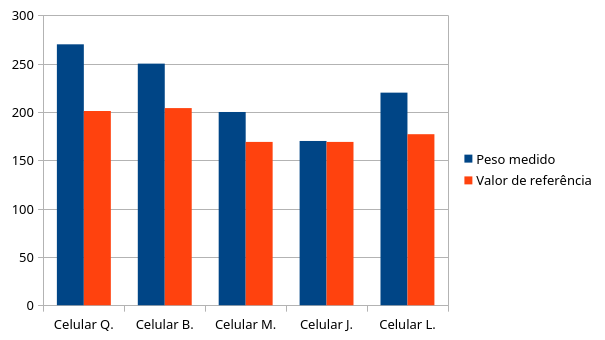
\includegraphics[width=.5\linewidth]{fig/pesos.png}
    \caption{Distribuição de peso e comparação com referência}
    \label{pesos}
\end{figure}
Note, inclusive, que o peso medido do Celular J. possui a melhor aproximação de
seu valor de referência, o que contribui com a hipótese de que o erro está
fortemente associado ao uso das capas protetoras, tendo em vista que este
aparelho foi o único pesado sem capa.
\subsection{Gangorra}

\subsection{Bonecos flutuantes}
O comportamento do boneco dentro da garrafa pode ser explicado pelos princípios
da hidrostática e da variação de pressão. Já sabemos, que o boneco flutuante possui uma
cavidade com ar em sua parte inferior, o que garante sua flutuação inicial
devido ao volume deslocado de água, que gera empuxo maior que o peso do boneco.
Quando a garrafa é pressionada, a pressão hidrostática no interior do líquido
aumenta, comprimindo o ar dentro do boneco e reduzindo seu volume de água
deslocado. Consequentemente, o empuxo diminui, fazendo com que o boneco desça.
Em relação ao boneco não-flutuante, a quantidade inicial de ar em sua cavidade
é menor e, consequentemente, sua força empuxo é menor. Nesse caso, a força
empuxo é menor que a força peso e, assim, o boneco não flutua mesmo sem aumento
da pressão externa. Dessa forma, observou-se que para vencer o desafio
proposto era necessário utilizar os ganchos no boneco flutuante para segurar o
boneco não-flutuante, que foi possível pois a soma das forças de empuxo dos
bonecos era superior a soma de suas forças peso.

Além disso, quanto à posição em que a garrafa é apertada, não há diferença
aparente no movimento do boneco, dado que, de acordo com o Princípio de Pascal,
a pressão aplicada em um fluido incompressível se transmite integralmente em
todas as direções. Portanto, independentemente do local onde se pressiona a
garrafa, a variação de pressão será a mesma em todo o sistema, resultando no
mesmo efeito sobre o boneco.
